
%(BEGIN_QUESTION)
% Copyright 2009, Tony R. Kuphaldt, released under the Creative Commons Attribution License (v 1.0)
% This means you may do almost anything with this work of mine, so long as you give me proper credit

Sketch the curve of a function that is the {\it derivative} of the function shown on the graph:

$$\includegraphics[width=15.5cm]{i04276x01.eps}$$

\vfil

\underbar{file i04276}
\eject
%(END_QUESTION)





%(BEGIN_ANSWER)

This is a graded question -- no answers or hints given!

%(END_ANSWER)





%(BEGIN_NOTES)

The derivative function will exhibit a {\it height} proportional to the {\it slope} of the given function.  Therefore, when the original function is level (flat), the slope is zero and therefore the derivative function will be on the $x$ axis (a value of 0).  When the original function is sloping upward, the derivative function will have a positive value.  When the original function is sloping downward, the derivative function will have a negative value:

$$\includegraphics[width=15.5cm]{i04276x02.eps}$$

%INDEX% Mathematics, calculus: derivative curve (sketching)

%(END_NOTES)


